% 
%  chapter6.tex
%
\chapter{Module Evaluation}~\label{ch:eval}
In this chapter, the evaluation and testing methodology of each module that make up CASCIFFO are detailed.
The chapter has the following structure:
\begin{enumerate}
    \item Back-End Evaluation~\ref{ch:eval:sec:be-eval};
    \item Front-End Evaluation~\ref{ch:eval:sec:fe-eval}.
\end{enumerate}

\section{Back-End Evaluation}\label{ch:eval:sec:be-eval}

The back-end module evaluation consisted in assuring that each layer (controller, service and repository) was functioning properly. To achieve this, several integration tests where made utilizing the \textit{Spring Unit}~\cite{spring-testing-unit} testing framework, the integration tests used an in-memory database based on \textit{H2}~\cite{h2-db} so that they could run without affecting the development database. The configurations required to set up this in-memory database require a different set of configurations compared to when using the main database. This can be achieved by creating another \texttt{.properties} file with its name set to \texttt{application-test}, thus creating the file \lstinline{application-test.properties}, a snippet of which can be viewed in listing~\ref{lst:spring-h2-config}. The striking differences are apparent in the properties \lstinline{spring.r2dbc.url}, \lstinline{spring.r2dbc.username} and \lstinline{spring.sql.init.data-locations}. The first two are now set to the configurations of the \textit{H2}, while the last one indicates where the testing data is located.

\begin{lstlisting}[
caption={Spring properties configurations with H2 database.},
label={lst:spring-h2-config}
]
# Database settings
spring.r2dbc.url=r2dbc:h2:mem:///~/test;MODE=PostgreSQL;
spring.r2dbc.username=SA
spring.sql.init.schema-locations=classpath:sql/schema.sql
spring.sql.init.data-locations=classpath:sql/data-h2-test.sql
\end{lstlisting}

In addition to the changes of the configuration file, we also require new testing libraries on the project, namely \textit{H2}, \textit{Spring Boot} and coroutines testing libraries. With this goal in mind, the following dependencies in listing~\ref{lst:spring-test-config} were added to the \lstinline{build.gradle.kt} file.

\begin{lstlisting}[
caption={Spring test dependencies snippet.},
label={lst:spring-test-config}
]
dependencies {
    // implementation and runtimeOnly dependencies...
    // test dependencies.
    testImplementation("io.r2dbc:r2dbc-spi:1.0.0.RELEASE")
    testImplementation("com.h2database:h2:2.1.214")
    testImplementation("io.r2dbc:r2dbc-h2:1.0.0.RELEASE")
    testImplementation("org.springframework.boot:spring-boot-starter-test:3.0.0")
    testImplementation("io.projectreactor:reactor-test:3.4.24")
}
testImplementation ("org.jetbrains.kotlinx:kotlinx-coroutines-test:1.6.4")
\end{lstlisting}

In order to start \textit{H2}~\cite{h2-db}, assuming it is installed, the service needs to be launched and afterwards it should automatically open a browser and direct the user to a localhost URL that initially may display an unsafe warning. This warning can be ignored since it is running on the local machine, not remotely. Upon advancing, the user is met with a login screen, here we can configure the credentials according to the previously created configurations, resulting in the settings which can be observed in figure~\ref{fig:h2-login-config}.

\begin{figure}[H]
    \centering
    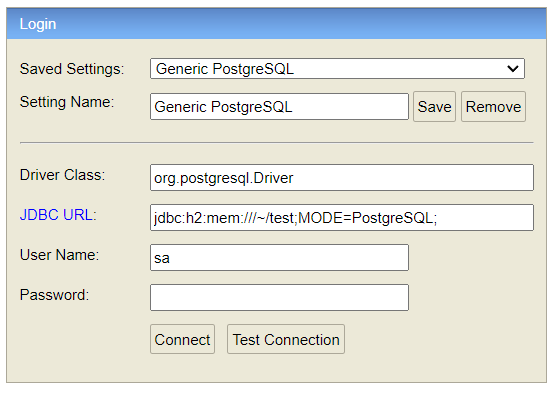
\includegraphics{Chapters/img/misc/h2-login-config.png}[scale=0.5]
    \caption{H2 configurations.}
    \label{fig:h2-login-config}
\end{figure}

With the database created and configured, the next step consists in creating the test classes. In order for these classes to use the different application properties, the annotation \lstinline{@ActiveProfiles(value = ["test"])} was be used to declare which Spring profile the application will use when loading the application context for test classes~\footnote{https://docs.spring.io/spring-framework/docs/current/javadoc-api/org/springframework/test/context/ActiveProfiles.html}. In addition, to launch the tests with the required application context with Spring Boot and provide other features, the annotation \lstinline{@SpringBootTest}~\footnote{https://docs.spring.io/spring-boot/docs/current/api/org/springframework/boot/test/context/SpringBootTest.html} was also used. A test file was created for each component with several methods testing the control flow and logic of their respective component. Since the application environment is non-blocking, two approaches were used to implement the tests. The first consists in using the \lstinline{StepVerifier} utility class, provided in the Project Reactor library that includes utility test methods that assert the behavior of reactive data streams of \lstinline{Mono} and \lstinline{Flux}. This is especially useful for testing the repository component, for example, in the listing~\ref{lst:test-proposal-repo}, we verify the correct verification of a proposal entity. Through several methods available in the utility class \lstinline{StepVerifier}, the entire behavior of the data stream can be tested. It is important to have each \lstinline{StepVerifier} block run the method \lstinline{.expectSubscription()} to subscribe to the stream passed as argument.

\begin{lstlisting} [
language={kt},
caption={Test method for the Proposal Repository.},
label={lst:test-proposal-repo}
]
 @Test
fun whenProposalCreated_thenFindIdInRepository() {
    val proposal = ProposalModel(
        sigla = "Created for test",
        type = ResearchType.OBSERVATIONAL_STUDY,
        stateId = 1,
        principalInvestigatorId = 1,
        therapeuticAreaId = 1,
        serviceTypeId = 1,
        pathologyId = 1
    )

    StepVerifier
        .create(proposalRepository.save(proposal))
        .expectSubscription()
        .`as`("Create proposal")
        .consumeNextWith {
            assert(it.id !== null)
            proposal.id = it.id
        }
        .expectComplete()
        .log()
        .verifyThenAssertThat()

    StepVerifier
        .create(proposalRepository.findById(pId = proposal.id!!))
        .expectSubscription()
        .`as`("Find created proposal with id ${proposal.id}")
        .thenAwait()
        .assertNext {
            it.id === proposal.id
        }
        .expectComplete()
        .log()
        .verifyThenAssertThat()
}   
\end{lstlisting}

This approach was used to test the repository layer, as each repository returned reactive data streams.

The second approach which was used to test the service layer, consisted in realizing the test inside a coroutine with the keyword \lstinline{runBlocking} which runs a coroutine in a blocking manner, meaning that the code inside it will be executed synchronously and will block the current thread until the coroutine completes, an example of this can be observed in listing~\ref{lst:test-add-patient-service}. It is important to note that this approach was used since the service layer heavily relies on \textit{Kotlin coroutines}.

\begin{lstlisting}[
language={kt},
caption={Unit integration test for adding a patient to an on-going research.},
label={lst:test-add-patient-service}
]
@Test
fun testServiceAddPatientToResearch() {
    var patient = PatientModel(
        processId = 102,
        fullName = "Manuel Santos",
        gender = "m",
        age = 50
    )
    runBlocking {
        patient = patientService.save(patient)
        val addedPatient = participantService.addPatientToResearch(patientId = patient.id!!, researchId = 1)
        val patients = patientService.findAllByResearchId(researchId = 1)
        assertDoesNotThrow {
            patients.first { assert(it.id === addedPatient.id) }
        }
    }
}
\end{lstlisting}

Finally the controller layer was tested using an external tool called \textit{Postman}~\cite{postman}. This platform allows the user to verify the responses and facilitate the ability to manipulate the header requests as well as viewing the response headers. The Postman request collection is available within the \textit{Github} repository.
Within Postman there are several fields we can define to build a request and receive a response, as viewed in the figure~\ref{fig:postman-post-req} which depicts a login request. This is a POST request made to the application running in localhost, hence the localhost URL which is defined with the variable \lstinline{localhost} surrounded by curly braces, along with the request body specifying the credentials of the user. Upon executing the request, the response received is also detailed the figure, consisting of the access token of the user, their roles, user id and user name.

\begin{figure}[H]
    \centering
    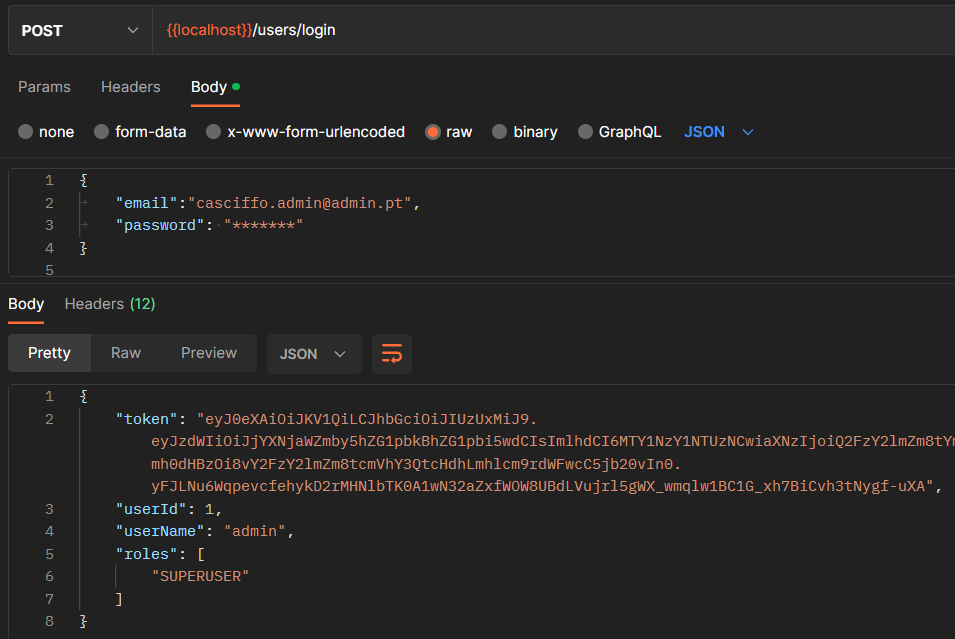
\includegraphics[scale=0.5]{Chapters/img/misc/postman-req-post.png}
    \caption{Authentication request made in Postman.}
    \label{fig:postman-post-req}
\end{figure}


\section{Front-End Evaluation}~\label{ch:eval:sec:fe-eval}

The \acrshort{fe} module evaluation consisted in the frequent use of the application with the usage of the continuous development methodology. To measure browser performance, the developer tool \textit{Lighthouse} was utilized to point out possible issues. 